\documentclass[10pt,pdf,hyperref={unicode}]{beamer}
\usepackage[utf8]{inputenc}
\usepackage[T1,T2A]{fontenc}
\usepackage[english, russian]{babel}
\usepackage{graphicx}
\usetheme{Rochester}

\title{\huge Отчет по заданию №2}
\author{Данько Артем, Шматенко Дарья, Ковалева Василина}
\date{Апрель 2019}

\begin{document}
\frame[plain]{\titlepage}

\section{Анализ}

\begin{frame}
\frametitle{Количество произведенного и сломавшегося оружия}
\framesubtitle{Для каждой из компаний за все месяцы сотрудничества}
\begin{figure}[t]
    \centering
    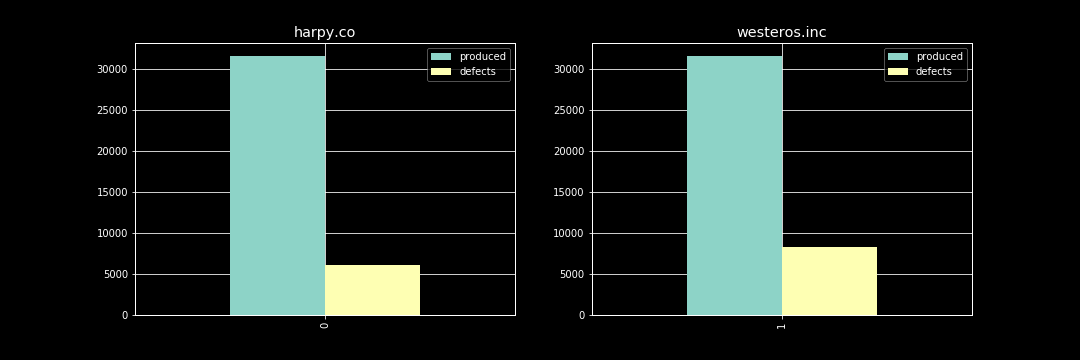
\includegraphics[width=1.0\textwidth]{6.png}
\end{figure}
Из графика видно, что за все время работы с поставщиками стали, количество произведенного оружия для обеих компаний почти совпадает. Однако число сломанных мечей компании Westeros Inс. заметно больше, чем у Harpy \& Co.
\end{frame}

\begin{frame}
\frametitle{Количество произведенного и сломавшегося оружия}
\framesubtitle{У обеих компаний для каждого месяца производства}
\begin{figure}[t]
    \centering
    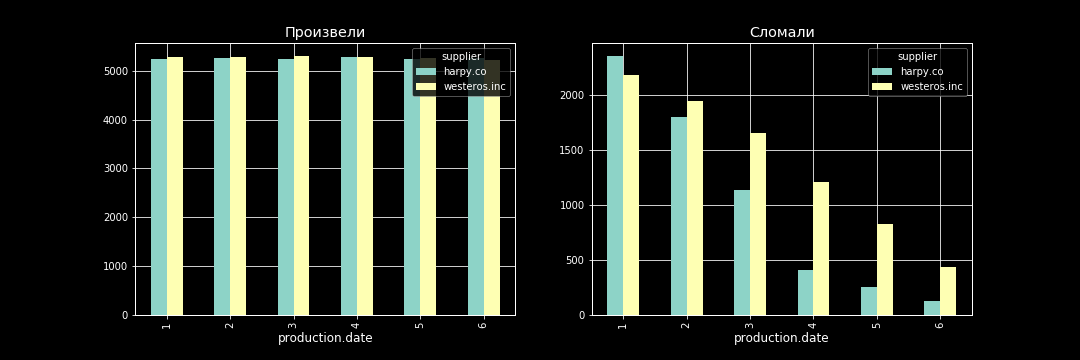
\includegraphics[width=1.0\textwidth]{3.png}
\end{figure}
Как и на предыдущем графике, число произведенного оружия за каждый месяц для этих компаний приблизительно равно. Тем не менее, качество стали Harpy \& Co заметно улучшилось в сравнении с Westeros Inс..
\end{frame}

\begin{frame}
\frametitle{Среднее число поломанной продукции}
\framesubtitle{Для каждого месяца производства}
\begin{figure}[t]
    \centering
    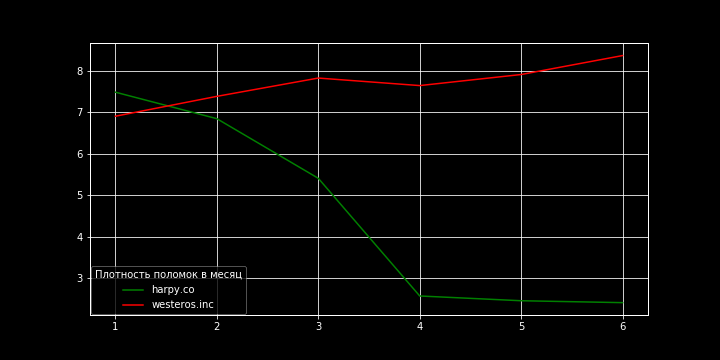
\includegraphics[width=0.8\textwidth]{4.png}
\end{figure}
Качество стали Harpy \& Co заметно улучшилось по сравнению с начальными результатами. В то время как мечи из стали Westeros Inс. в среднем стали ломаться чуть больше к шестому месяцу.
\end{frame}

\begin{frame}
\frametitle{Среднее число поломанной продукции}
\framesubtitle{По сроку службы}
\begin{figure}[t]
    \centering
    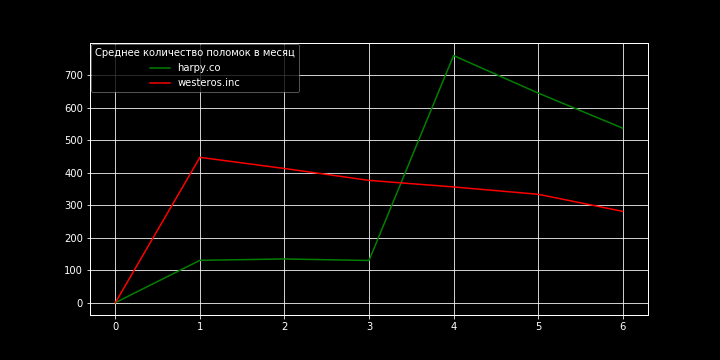
\includegraphics[width=0.8\textwidth]{1.png}
\end{figure}
Количество мечей, сломавшихся уже после первого месяца эксплуатации, у компании Westeros Inс. значительно превосходит Harpy \& Co. Однако, начиная с четвертого месяца использования, мечи, произведенные из стали Harpy \& Co, ломаются чаще.
\end{frame}
\section{Выводы}

\begin{frame}
\frametitle{Качество продукции за каждый месяц}
\begin{figure}[t]
    \centering
    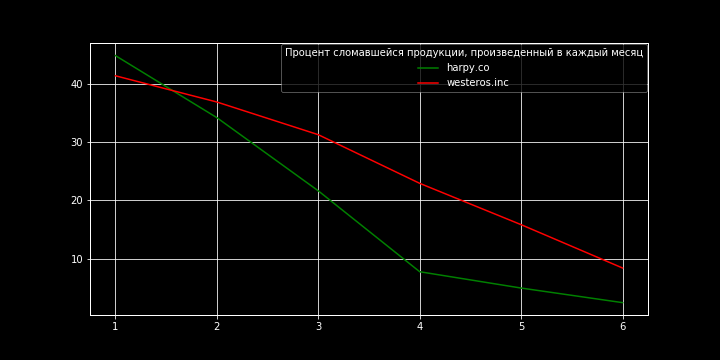
\includegraphics[width=0.8\textwidth]{2.png}
\end{figure}
График демонстрирует процентное соотношение сломанной и произведенной продукции за каждый месяц. К последнему месяцу закупки стали у обоих поставщиков, доля сломанных изделий снижается у обеих компаний.
\end{frame}

\begin{frame}
\frametitle{Зависимость количества поломок от кузнеца}
\begin{figure}[t]
    \centering
    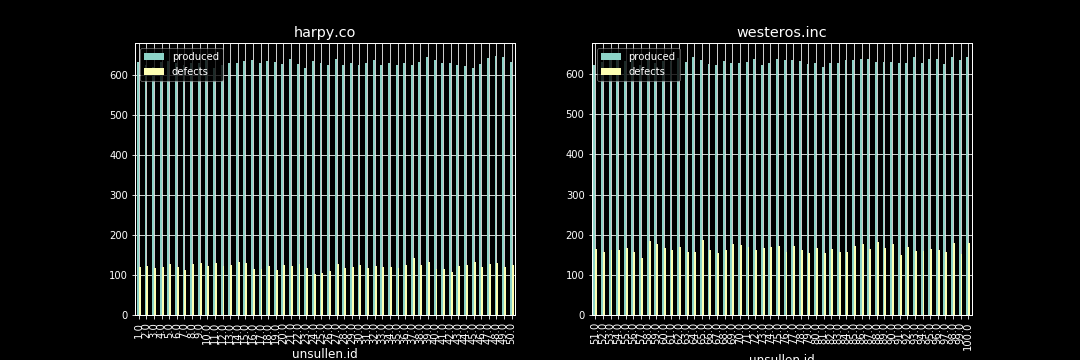
\includegraphics[width=1.0\textwidth]{5.png}
\end{figure}
Как видно из графика, количество сломанных и произведенных мечей для кузнецов в каждой из компаний находится на одинаковом уровне.
\end{frame}

\section{Выводы}

\begin{frame}
\frametitle{\insertsection}
    \begin{itemize}
        \item По результатам анализа качество стали компании Harpy \& Co выше, чем у Westeros Inс.
        \item Все кузнецы у каждой из компаний одинаково квалифицированы. 
        \item Поломка мечей зависит исключительно от качества стали.
    \end{itemize}
    
    \begin{block}{Итоги}
    Обобщая вышесказанное, мы приходим к выводу, что следует заключить эксклюзивный договор на поставку стали с компанией Harpy \& Co.
    \end{block}
\end{frame}

\end{document}
